%!TeX root=../tese.tex
%("dica" para o editor de texto: este arquivo é parte de um documento maior)
% para saber mais: https://tex.stackexchange.com/q/78101/183146

\chapter{Benchmarks}
\label{chap:benchmarks}

\section{Metodologia}
Os algoritmos foram implementados na linguagem C++ usando apenas as bibliotecas
padrão e a STL. Todos os programas foram compilados com a versão 7.4.0 do
compilador g++, num computador que possui um processador Intel Core i5-8250U
com clock base de 1.60GHz e turbo boost até 3.40GHz em uma única thread. As medições
de tempo foram feitas com o \texttt{steady\_clock} da biblioteca \texttt{<chrono>},
utilizando uma precisão de nanosegundos, tomando o devido cuidado de cronometrar apenas
as partes relevantes do código. Todos os programas foram compilados com a flag
\texttt{-O2} para permitir otimizações por parte do compilador.

Para cada algoritmo apresentado neste trabalho, foram medidos os tempos de execução tanto
da parte de preprocessamento quanto da parte de consultas, separadamente. Cada teste
também foi realizado com árvores lineares, binárias e quaternárias para evidenciar 
possíveis diferenças de performance de acordo com o formato da árvore.

Todas as árvores geradas para fins destes testes são completas (portanto balanceadas) 
e seus tamanhos variaram entre 150K e 21.6M. Tanto os testes de preprocessamento quanto
os de consultas foram executados dez vezes com cada tamanho de árvore para tomar então
suas médias como resultado. 

Os testes de preprocessamento consistem em um programa que cria uma árvore completa
com a quantidade de nós e o fator de ramificação desejados e então cria um objeto da
classe associada ao algoritmo a ser testado, o que equivale à fase de preprocessar a
árvore de entrada. Já os testes de consultas consistem em um programa que cria também
uma árvore completa com os mesmos parâmetros e então executam um conjunto de 10M de
consultas gerado previamente. Estes arquivos foram gerados aleatoriamente de forma que
toda consulta seja composta por um nó válido (entre 0 e $N-1$) onde $N$ é o tamanho do
experimento e uma profundidade válida (entre 0 e $profundidade(u)$), onde $u$ é o nó
da consulta.

\section{Análise dos resultados}
As árvores que surgiriam em aplicações reais possivelmente não seriam exatamente como
as árvores aqui testadas, que são todas completas, porém ainda podemos ter uma boa
noção de como as diferentes implementações se comportam no pior caso possível e em casos
mais favoráveis.

\subsection{Preprocessamento}

\subsubsection{Árvores lineares}
A primeira coisa a ser notada é que, para árvores lineares, o Algoritmo da Tabela mal
pode ser comparado com os outros, já que para este caso sua complexidade de espaço
de preprocessamento é $\bigO(n^2)$, se tornando impossível manter o programa na memória
até mesmo para o menor tamanho de árvore, 150K. Apesar disso, não é interessante
diminuir as árvores para que os testes não se tornem facilmente influenciáveis por
fatores do sistema como trocas de contexto, por exemplo.

Como esperado, o algoritmo da Preordem leva uma vantagem grande sobre o algoritmo dos
Ponteiros devido à diferença de complexidade entre eles e o Trivial se mantém
essencialmente constante, a menos de pequenas variações.

\begin{figure}
  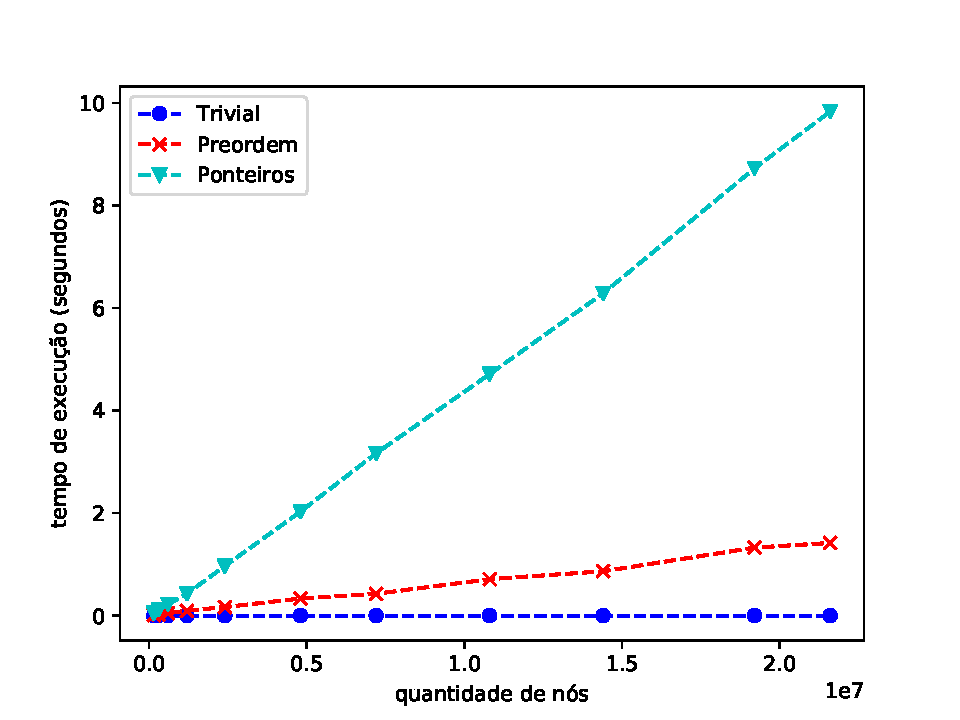
\includegraphics[scale=0.8]{preprocess_linear.pdf}
  \caption{Resultados para o preprocessamento de árvores lineares.}
\end{figure}

\newpage

\subsubsection{Árvores binárias}
Para estas árvores já é possível rodar o Algoritmo da Tabela para todos os tamanhos já
que sua complexidade de espaço agora é $\bigO(n \log n)$, sendo comparável com o
Algoritmo dos Ponteiros, que se mostrou menos eficiente. O Algoritmo da Preordem se tornou
ainda mais rápido, provavelmente por serem necessárias menos alocações de memória.

\begin{figure}
  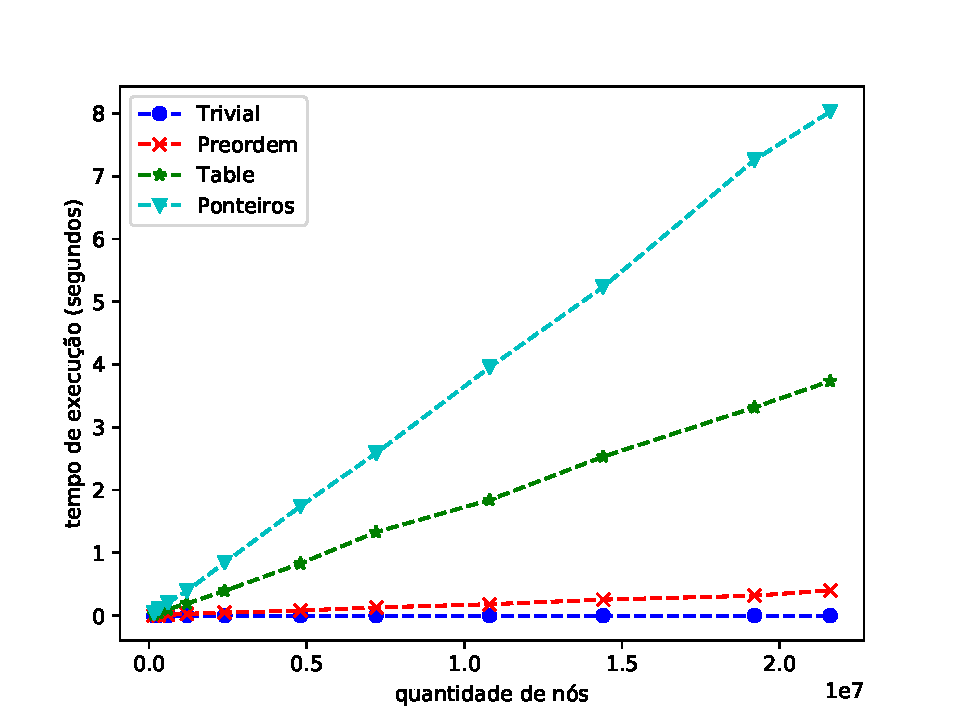
\includegraphics[scale=0.8]{preprocess_binary.pdf}
  \caption{Resultados para o preprocessamento de árvores binárias.}
\end{figure}

\subsubsection{Árvores quaternárias}
Para estas árvores é interessante notar que o desempenho do Algoritmo da Tabela foi
maior do que para árvores binárias e isso se deve à relação entre sua complexidade
de tempo e o fator de ramificação da árvore, já que esta é $\bigO(n \log_k n)$, onde
$k$ é o fator. O Algoritmo dos Ponteiros se manteve estável já que sua complexidade
não depende de $k$.

\begin{figure}[H]
  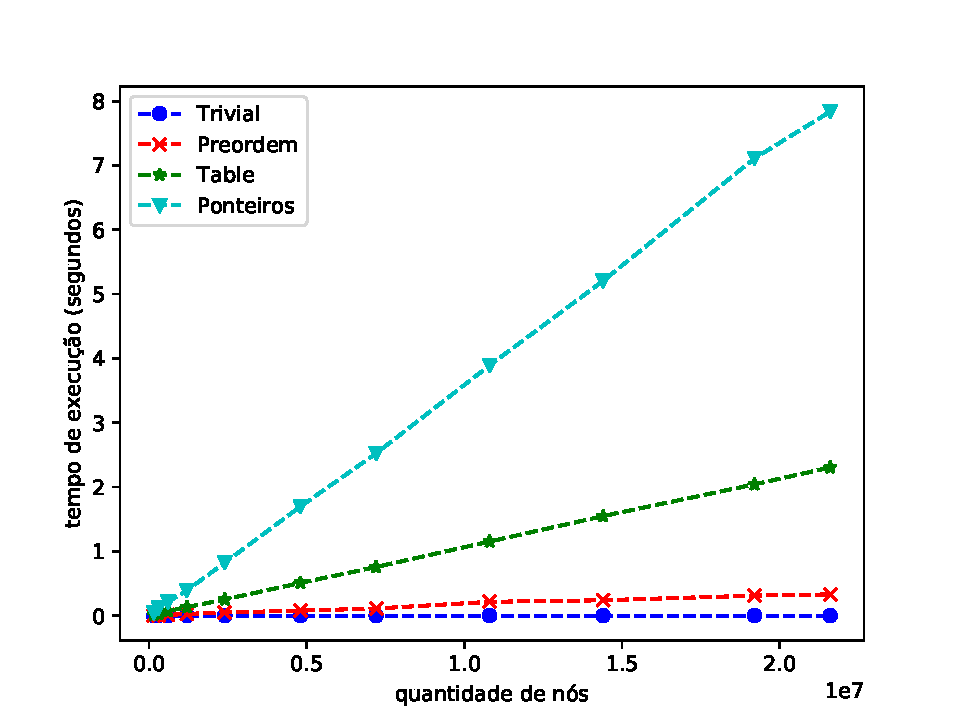
\includegraphics[scale=0.8]{preprocess_4ary.pdf}
  \caption{Resultados para o preprocessamento de árvores quaternárias.}
\end{figure}

\subsection{Consultas}

\subsubsection{Árvores lineares}
\subsubsection{Árvores binárias}

\begin{figure}[H]
  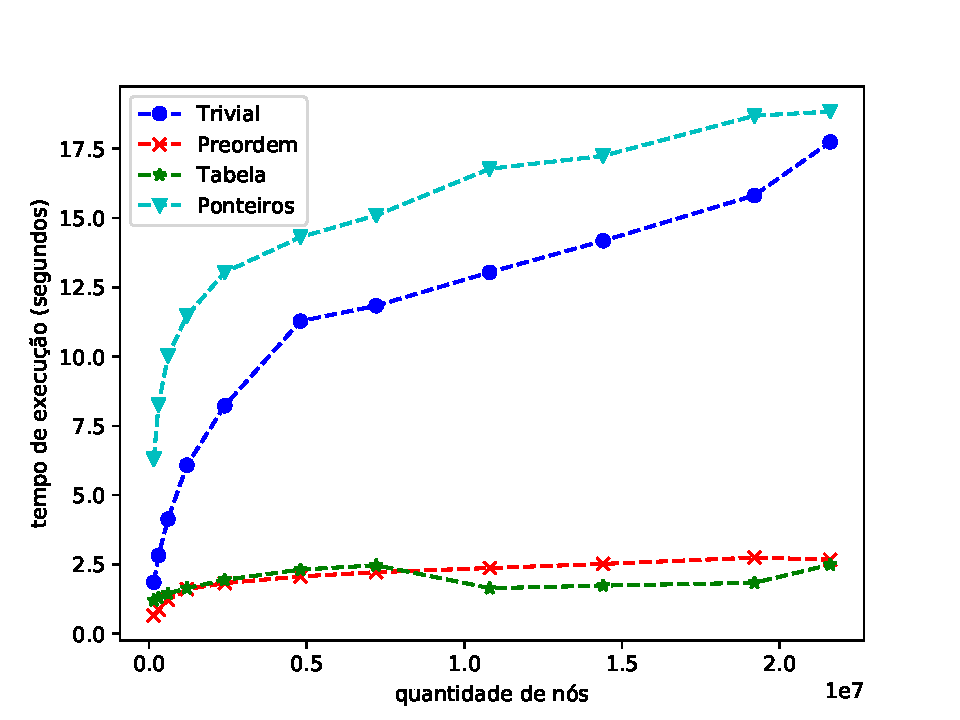
\includegraphics[scale=0.8]{query_binary.pdf}
  \caption{Resultados para as consultas em árvores binárias.}
\end{figure}

\subsubsection{Árvores quaternárias}

\begin{figure}[H]
  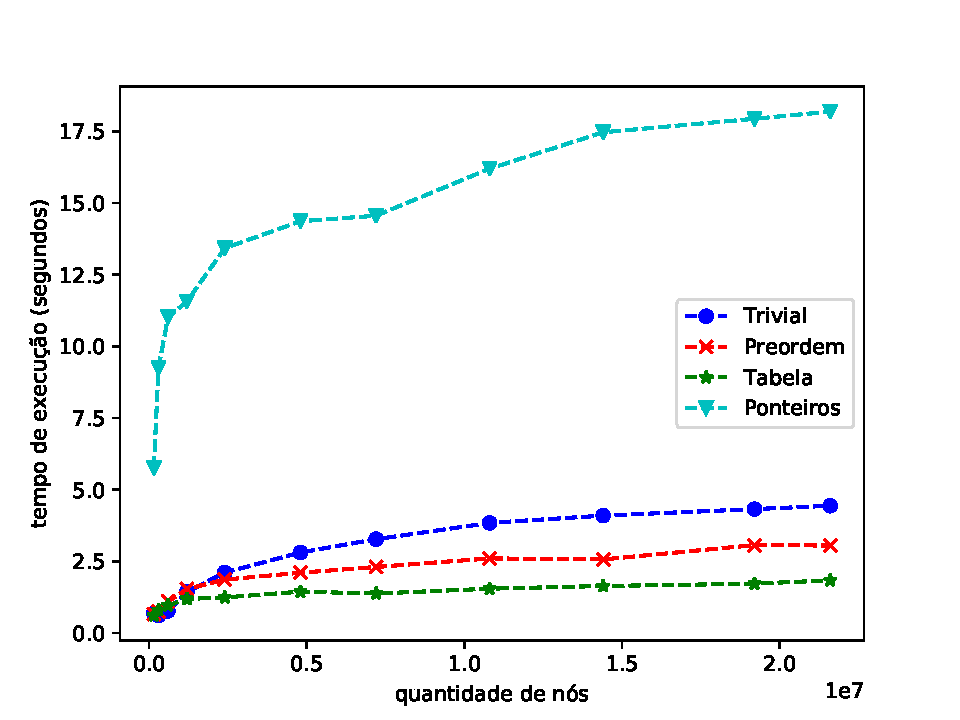
\includegraphics[scale=0.8]{query_4ary.pdf}
  \caption{Resultados para as consultas em árvores quaternárias.}
\end{figure}

\subsection{Conclusões}
Quase todos os algoritmos, exceto pelo algoritmo dos Ponteiros, se mostram mais
eficientes à medida que o fator de ramificação da árvore aumenta, já que isso causa
uma diminuição na sua profundidade esperada, que por sua vez tem relação direta com
a complexidade das implementações. É bastante interessante notar que implementações
simples como o algoritmo da Preordem e o da Tabela podem obter resultados muito
melhores do que outros mais complexos como o algoritmo dos Ponteiros. 